\subsection{Linear Least Squares Estimation}

\begin{figure}[htb]
\centering
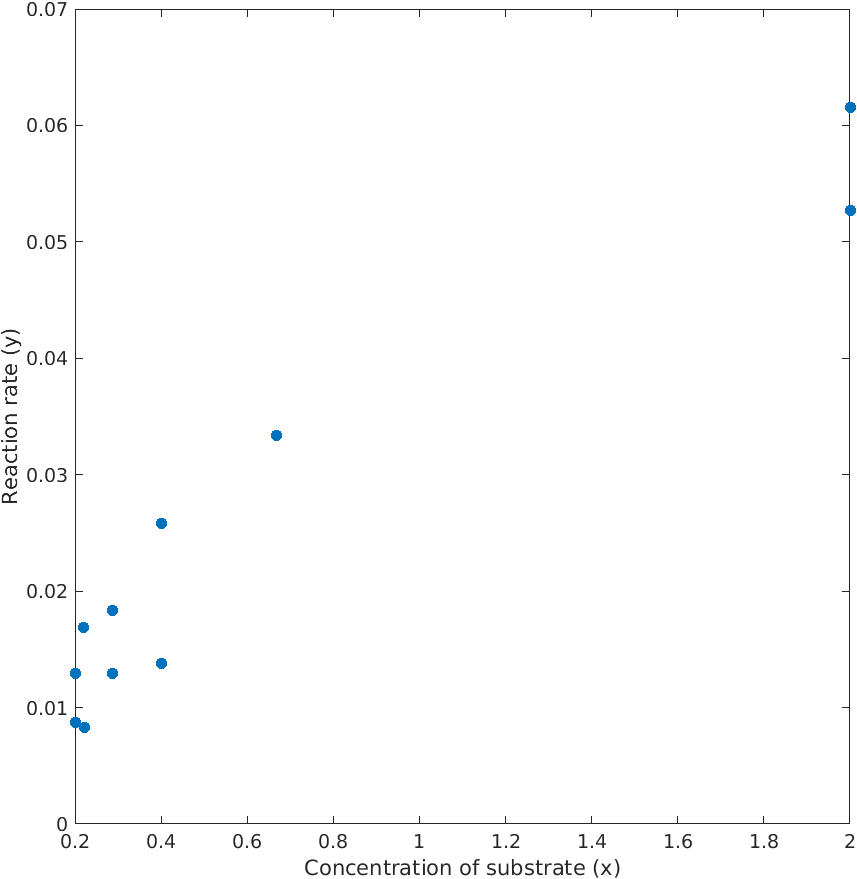
\includegraphics[width=0.6\textwidth]{../img/2-1raw}
\caption{}
\label{fig:2-1raw}
\end{figure}

The given data can be seen in figure \ref{fig:2-1raw}. In the following, Michaelis-Menten kinetics will be used as a model for the data:

\begin{equation}
y = \frac{\theta_1 x}{\theta2 + x}
\end{equation}

where $y$ is the reaction rate and $x$ is the concentration of the substrate. It should be noted that as

\begin{equation}
\lim_{x \rightarrow \infty} y = \theta_1
\label{limitEQ}
\end{equation}

and that for $x=\theta_2$

\begin{equation}
y = \frac{\theta_1 \theta_2}{\theta_2 + \theta_2} = \frac{\theta_1}{2}
\label{starting_guessEQ}
\end{equation}

This means that the maximum reaction rate is $\theta_1$, and that half of the maximum reaction rate is reached for $x = \theta_2$. We use this insight to set our starting guess for the optimal $\theta_1$ and $\theta_2$. We do this by letting the initial $\theta_1$ be equal to the largest $y$ value in the observed data, and letting the initial $\theta_2$ be equal to the $x$ value at which half of the highest reaction rate is achieved. This puts the initial guess at

\begin{equation}
\theta_0 = \begin{pmatrix}
0.0615 \\ 0.6670
\end{pmatrix} \label{eq:init}
\end{equation}

It should be expected, that these values are too low, as it does not seem from the raw data, that any plateau is reached for the highest concentration. Also following from this, it should be noted that both $\theta_1$ and $\theta_2$ are positive, as negative values could result in a negative reaction rate, which is not sensible as the model is based on an irreversible reaction transforming substrate to product. This is used as bounds for the algorithms, such that $(\begin{smallmatrix} 0 \\ 0 \end{smallmatrix}) \leq (\begin{smallmatrix} \theta_1 \\ \theta_2 \end{smallmatrix})$


\begin{figure}[htb]
\centering
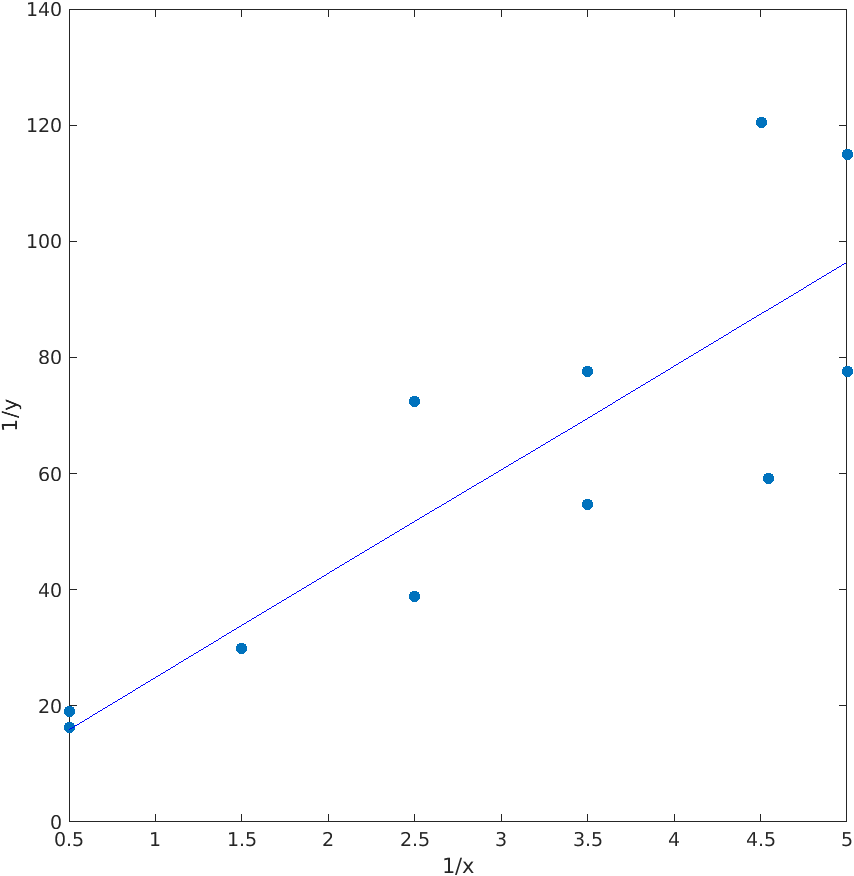
\includegraphics[width=0.6\textwidth]{../img/2-1reciprocal}
\caption{This plot shows the fitted linear least squares model, $\theta^{*}_{LS}$, and its predictions against the observational data. Note that the axes are based on the reciprocal of the data. }
\label{fig:2-1reciprocal}
\end{figure}

\paragraph{Linear estimation} To transform the problem into a linear least squares problem, two variables are introduced as



\[
a = \frac{1}{x} \quad \text{and} \quad b = \frac{1}{y}
\]

with these inserted the model can be written as

\[
b = \frac{\theta_2 + x}{\theta_1 x} = \frac{\theta_2 + \frac{1}{a}}{\theta_1} a = \frac{\theta_2}{\theta_1} a + \frac{1}{\theta_1}
\]

such that a line can be estimated with slope $\alpha = \frac{\theta_2}{\theta_1}$ and intercept $\beta = \frac{1}{\theta_1}$.

By letting $\mathbf{a}$ be a vector of the reciprocal of each observed substrate concentration, and $\mathbf{b}$ be a vector of the reciprocal of the observed reaction rate, the minimization problem can be written as a least squares problem

\[
\min_{\mathbf{p} \in \mathbb{R}^2} \left\Vert \mathbf{A} \mathbf{p} - \mathbf{b} \right\Vert_2^2
\]

where

\[
\mathbf{A} = \begin{pmatrix}
\mathbf{a} & \mathbf{1}
\end{pmatrix} \quad \text{and} \quad
\mathbf{p} = \begin{pmatrix}
\alpha \\ \beta
\end{pmatrix}
\]

This is a quadratic problem, as

\begin{align}
\left\Vert \mathbf{A} \mathbf{p} - \mathbf{b} \right\Vert_ 2^2 &= (\mathbf{A} \mathbf{p} - \mathbf{b})^T (\mathbf{A} \mathbf{p} - \mathbf{b}) \\
&= \frac{1}{2} \mathbf{p}^T (2 \mathbf{A}^T \mathbf{A}) \mathbf{p} + (-2\mathbf{A}^T b)^T \mathbf{p} + \mathbf{b}^T \textbf{b} \\
&= \frac{1}{2} \mathbf{p}^T \mathbf{H} \mathbf{p} + \mathbf{g}^T \mathbf{p} + \mathbf{b}^T \textbf{b}
\end{align}

This is solved in \matlab using \texttt{quadprog} giving parameters $\alpha = 17.8738$ and $\beta = 7.0247$. The reciprocal data can be seen with the linear model in figure \ref{fig:2-1reciprocal}. Backtransforming the parameters gives

\[\theta^{*}_{LS} = \lbrace
\theta_1 = \frac{1}{\beta} = 0.1424\quad \text{and}  \quad
\theta_2 = \alpha \theta_1 = 2.5444\rbrace
\]

where we denote $\theta^{*}_{LS}$ our linear least squares estimate. Figure \ref{fig:2-1reciprocal} below shows the least squares model with the reciprocal data. 

\begin{figure}[htb]
\centering
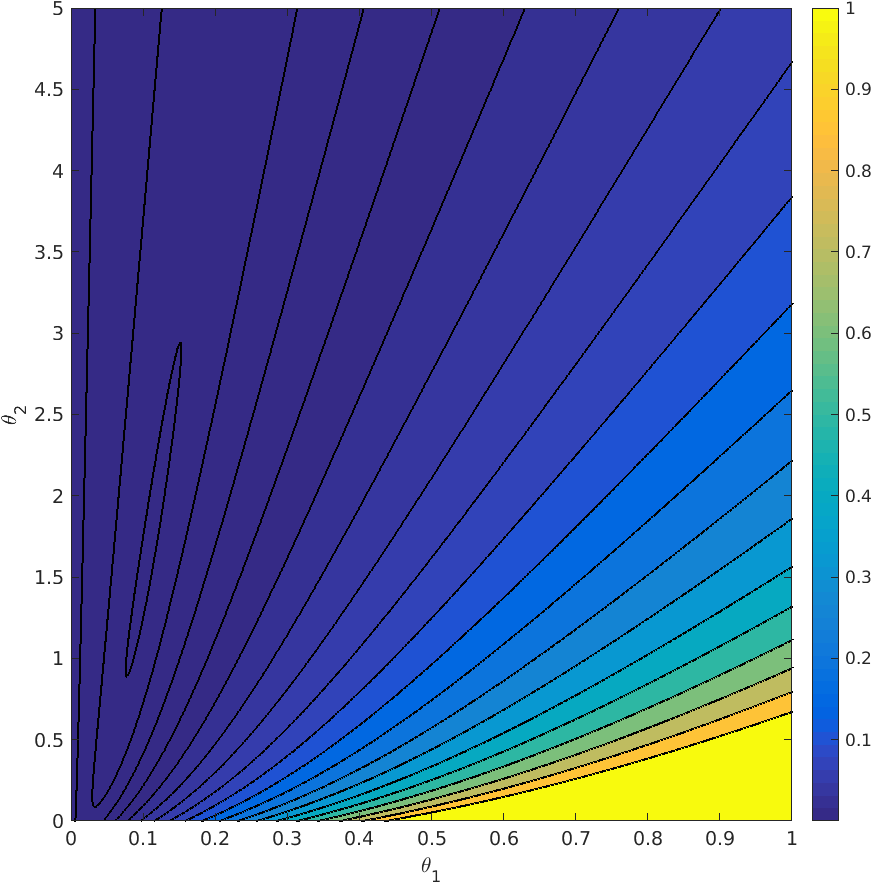
\includegraphics[width=0.6\textwidth]{../img/2-2phi}
\caption{This plot shows the magnitude of the residuals as contours resulting from different combinations of $\theta_1$ and $\theta_2$. Deep blue colors represent low residual values where optimal theta estimates can be found. Note that only the positive quadrant is shown as the solution is to be positive.}
\label{fig:2-2phi}
\end{figure}

\subsection{Nonlinear Optimization}

\paragraph{Nonlinear estimation}
When doing the transformation to a linear problem, it is still assumed that the reciprocals are normally distributed afterwards when fitting the model. If the reciprocals are in fact normally distributed before the transformation, they won't be afterwards (the reciprocal of a normal distribution will be a bimodal distribution). To avoid this, a model can be fitted without transforming it by using nonlinear optimization

\begin{equation}
\min_{\theta \in \mathbb{R}^2} \phi(\theta) = \frac{1}{2} \sum_{i=1}^{m} \left\Vert y_i - f(\theta, x_i)\right\Vert_2^2
\end{equation}

where $\theta = \begin{pmatrix}
\theta_1 \\ \theta_2
\end{pmatrix}$ and $f(\theta, x) = \frac{\theta_1 x}{\theta_2 + x}$. 

\begin{table}[htb]
\centering
\small
\begin{tabular}{l|cccc} \hline \hline 
Algorithm & $\phi$ & Time [ms] & Iterations & Funciton calls  \\ \hline\texttt{quadprog} & 1.348e-04 & 4.4 & 3 & - \\ 
\texttt{nonlinsq} & 9.539e-05 & 15.8 & 3 & 12 \\ 
\texttt{nonlinsq} with Jacobian & 9.539e-05 & 11.3 & 3 & 4 \\ 
\hline \hline 
\end{tabular} 

\caption{The time is calculated as an average over 100 repetitions. The \texttt{quadprog} algorithm does not return a number of function calls.}
\label{tab:2comparison}
\end{table}

A section of the contours of $\phi(\theta)$ can be seen in figure \ref{fig:2-2phi}. Note that we only show the positive quadrant as the solution has to be positive. It is seen that the lowest values of $\phi(\theta)$ are in the area of $\theta_1 \in [0.07; 0.15]$ and $\theta_2 \in [0.9; 3]$ (the ellipsoid contour line). This is indeed a little higher than the initial estimate ($\theta_0 = \begin{psmallmatrix}
0.0615 \\ 0.6670
\end{psmallmatrix}$) discussed in the first section. 

\begin{figure}[htb]
\centering
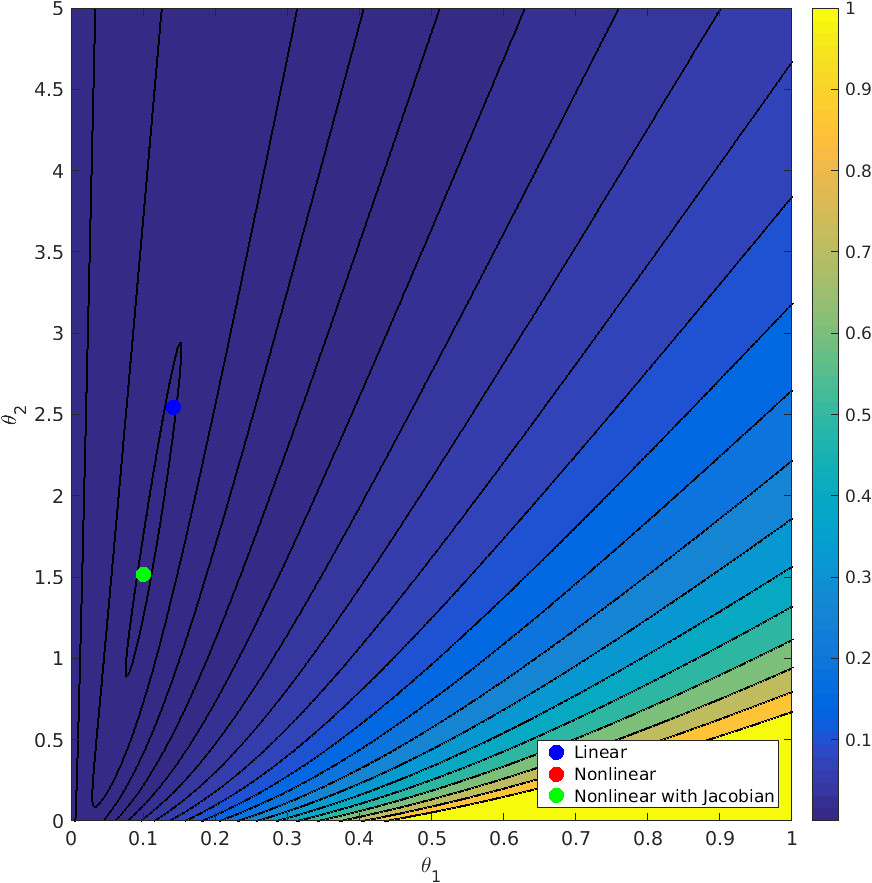
\includegraphics[width=0.6\textwidth]{../img/2-2phiPoints}
\caption{The estimated solutions $\theta^{*}_{LS}$ (blue dot) and $\theta^{*}$ (green dot) are shown. Note that the estimated $\theta^{*}$ with and without the Jacobian are identical, and therefore are overlapped in the plot - only one can be seen.}
\label{fig:2-2phiPoints}
\end{figure}

As this is a least squares problem, we solve it using the \texttt{lsqnonlin} function in \matlab. We denote this parameter solution as $\theta^*$. We solved it with and without supplying the Jacobian to the function to compare computational efficiency. Table \ref{tab:2comparison} lists the computational efficiency results for \texttt{quadprog} (the linear case), and for \texttt{nonlinsq} (the nonlinear case) with and without the Jacobian. It is evident that in regards to speed \texttt{quadprog} (4.4 msec) is more than three times faster than \texttt{nonlinsq} wihout the Jacobian (15.8 msec). And as expected, supplying the Jacobian eases the calculation, and indeed we see a 28\% reduction in computational time needed to derive the solution as well as 66\% less function calls (see Table \ref{tab:2comparison}). 



\begin{table}[htb]
\centering
\small
\begin{tabular}{l|ccc|cc} \hline \hline 
\multicolumn{6}{c}{Linear estimation} \\ \hline \hline
Parameter & Estimate & Lower bound & Upper bound & \multicolumn{2}{c}{Covariance}  \\& & & & $\theta_1$ & $\theta_2$ \\ \hline 
$\theta_1$ & 0.14 & 0.06 & 0.22 & 0.00 & \\ 
$\theta_2$ & 2.54 & 0.43 & 4.66 & 0.03 & 0.90 \\ 
\hline \hline 
\multicolumn{6}{c}{Nonlinear estimation} \\ \hline \hline
Parameter & Estimate & Lower bound & Upper bound & \multicolumn{2}{c}{Covariance}  \\& & & & $\theta_1$ & $\theta_2$ \\ \hline 
$\theta_1$ & 0.10 & 0.07 & 0.13 & 0.00 & \\ 
$\theta_2$ & 1.51 & 0.66 & 2.37 & 0.01 & 0.15 \\ 
\hline \hline 
\multicolumn{6}{c}{Nonlinear estimation with Jacobian} \\ \hline \hline
Parameter & Estimate & Lower bound & Upper bound & \multicolumn{2}{c}{Covariance}  \\& & & & $\theta_1$ & $\theta_2$ \\ \hline 
$\theta_1$ & 0.10 & 0.07 & 0.13 & 0.00 & \\ 
$\theta_2$ & 1.51 & 0.66 & 2.37 & 0.01 & 0.15 \\ 
\hline \hline 
\end{tabular} 

\caption{The statistical characteristics of the parameter estimates of the different models are shown above. The lower and upper bounds represent the $95\%$ confidence intervals of parameter uncertainty.}
\label{tab:2NL}
\end{table}

Our results are plotted in Figure \ref{fig:2-2phiPoints}. The three methods ($\theta^{*}_{LS}$, and $\theta^*$ with and without the Jacobian) were started with the same initial guess ($\theta_0 = \begin{psmallmatrix}
0.0615 \\ 0.6670
\end{psmallmatrix}$). Recall from Section 2.1 that our initial starting guess was made based on the insights from equations \ref{limitEQ} and \ref{starting_guessEQ}, and which was relatively close to the minimum found on the countour plot. From this starting guess, all three methods took three iterations to converge to the points illustrated in \ref{fig:2-2phiPoints}. Both methods converged to the ellipsis of minimum residual value. It is worth noting, however, that while the linear estimation is more computationally efficient, the nonlinear estimation results in better uncertainty bounds and have a lower sum of squared residuals value. Table \ref{tab:2NL} shows the estimated parameters and their $95\%$ confidence intervals for both methods. The uncertainty in $\theta_1$ is reduced $66\%$ using nonlinear estimation relative to the linear estimation. Similarly, the parameter estimation uncertainty in $\theta_2$ is reduced by $42\%$. 

\begin{figure}[htb]
\centering
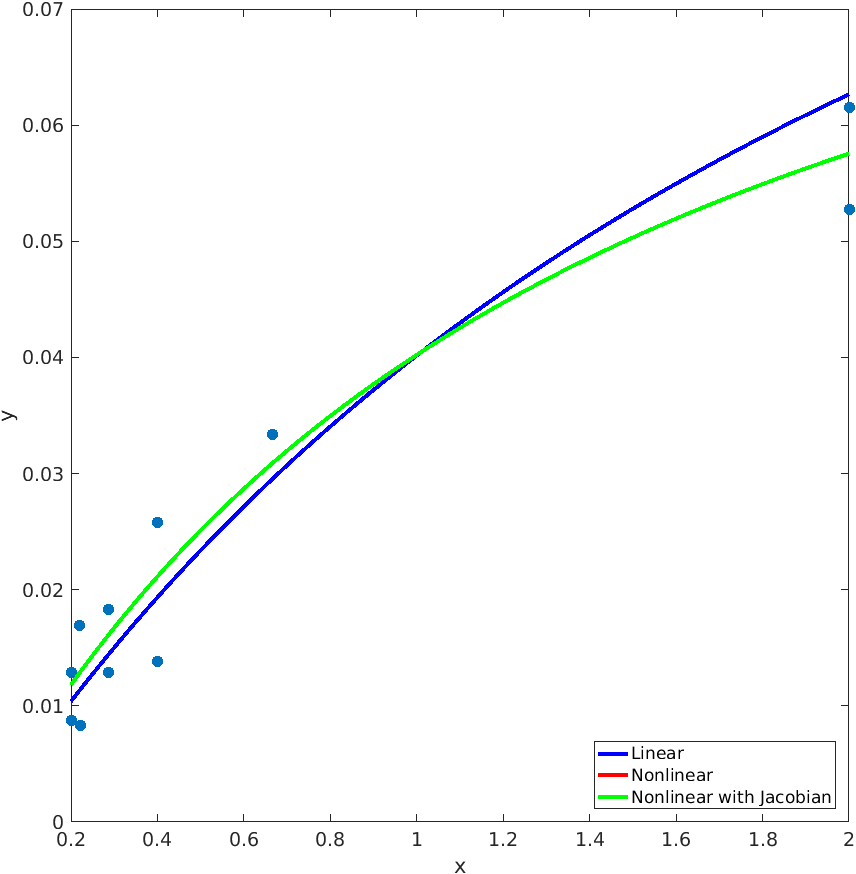
\includegraphics[width=0.65\textwidth]{../img/2-2est}
\caption{The linear and nonlinear fitted models and their predictions against the observational data are shown above. The x-axis represents the substrate concentration while the y-axis represents the reaction rate. Notice that the nonlinear model with and without the Jacobian are identical, and therefore one overlaps the other (i.e. only one can be seen).}
\label{fig:2-2est}
\end{figure}

Figure \ref{fig:2-2est} shows the linear and nonlinear models against the observational data. Both estimate similar $\theta_1$ values of $0.14$ and $0.10$, respectively. This is the asymptotic reaction rate of the model for large substrate concentration. In contrast, $\theta_2$ varies more between the two (see Table \ref{tab:2NL}) and results in slightly different slopes. Consequently, if we look at the highest substrate concentrations in the plot, we notice that the linear model "misses" the last two data observations while the nonlinear model better captures these two data points. This "miss" by the linear model presumably may stem from the fact that it was fitted with the reciprocal data (Figure \ref{fig:2-1reciprocal} shows a good fit in zones of high substrate concentration with the reciprocal data). Regardless, given the parameter uncertainty involved, it is likely that the linear model overestimates reaction rates in zones of high substrate concentration.   

To sum up, both methods converged to similar solutions. However, while the linear estimation was more computationally efficient using \texttt{quadprog}, the nonlinear estimation using \texttt{lsqnonlin} resulted in drastically better confidence bounds.  

\subsection{Time vs. Substrate concentration}

Instead of having the data as substrate concentration vs. reaction rate, a Michaelis-Menten model can be estimated from time vs. substrate concentration. This is useful because in practice the reaction rate is difficult to obtain. The \texttt{ModelAndSensitivity} script provided in Lecture 12 is used with \verb+n=1+ (number of initial conditions, which is only the substrate concentration), \verb+np=2+ (number of parameters, which is $\theta_1$ and $\theta_2$), \verb+xdot = -p(1)*x/(p(2)+x)+ (which is the Micaelis-Menten model for the reaction rate) and a function is made for the derivatives which returns the partial derivatives of $\frac{\theta_1 x}{\theta_2 + x}$ with respect to $x$, $\theta_1$ and $\theta_2$. 

The \texttt{ModelAndSensitivity} script is used for estimating the substrate concentration and the Jacobian using the \verb+ode45+ function, the residuals are found and are passed as input arguments to \verb+lsqnonlin+ along with the Jacobian to estimate the parameters $\theta_1$ and $\theta_2$. 

\begin{figure}[htb]
\centering
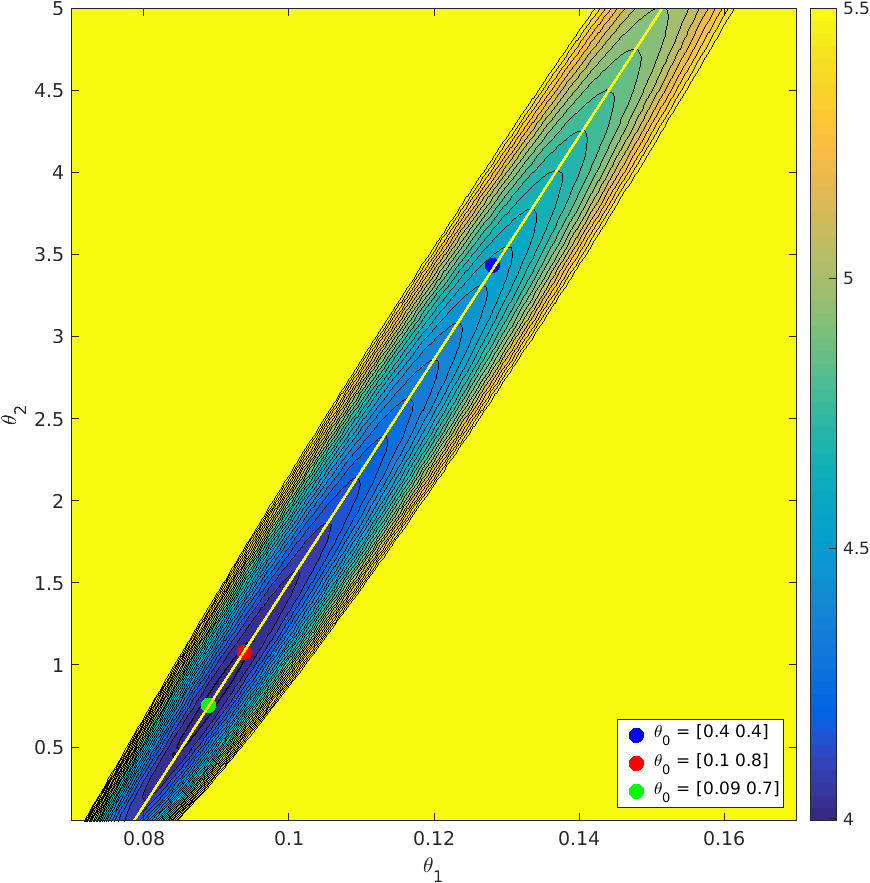
\includegraphics[width=0.55\textwidth]{../img/2-3Phi}
\caption{Solutions for Trust Region Reflective algorithm using Jacobian, with default parameters. Notice that the green and red dot converges to different solutions, even though they start close to each other.}
\label{fig:2-3Phi}
\end{figure}


We use the \verb+lsqnonlin+ algorithm because it is specifically suited for nonlinear least squares objectives. The \verb+lsqnonlin+ function has the option to choose between two numerical algorithms: Trust Region Reflective and Levenberg-Marquardt. The Trust Region Reflective (TRR) algorithm is better suited for problems with no constraints or with only bound constraints. In contrast, the Levenberg-Marquardt (LM) algorithm is unable to handle bound constraints and is better suited for underdetermined problems. That is, problems characterized by a system with less equations than unknown variables. Since our solution is bounded to positive values and the problem is not underdetermined, we opt for Trust Region Reflective algorithm in the \verb+lsqnonlin+ function options. For comparison purposes however, we solve using both numerical algorithms, (see Table \ref{tab:2-3} for results).    

\begin{table}[H]
\centering
\footnotesize
\begin{tabular}{ccc} \hline \hline 
\multicolumn{3}{c}{Trust Region Reflective} \\ \hline
$\theta_0$ 		& $\hat{\theta}$ 	& $\phi(\hat{\theta})$ \\ \hline
$[0.4\ 0.4]$ 	& $[0.128\ 3.43]$ 	& 4.56 \\
$[0.1\ 0.8]$  		& $[0.0938\ 1.08]$ 	& 4.01 \\ 
$[0.09\ 0.7]$	& $[0.0889\ 0.753]$ 	& 3.99 \\ \hline \hline
\multicolumn{3}{c}{Levenberg Marquardt} \\ \hline
$\theta_0$ 		& $\hat{\theta}$ 	& $\phi(\hat{\theta})$ \\ \hline
$[0.4\ 0.4]$		& $[4.00\ 4.00]$		& 128 \\ 
$[0.1\ 0.8]$		& $[0.0940\ 1.09]$	& 4.01 \\
$[0.09\ 0.7]$	& $[0.0890\ 0.752]$	& 4.00 \\ \hline \hline
\multicolumn{3}{c}{Tweaked Trust Region Reflective} \\ \hline
$\theta_0$ 		& $\hat{\theta}$ 	& $\phi(\hat{\theta})$ \\ \hline
$[0.4\ 0.4]$		& $[0.128\ 3.43]$	& 4.56	 \\ 
$[0.1\ 0.8]$  		& $[0.0938\ 1.08]$ 	& 4.01 \\ 
$[0.09\ 0.7]$	& $[0.0889\ 0.753]$ 	& 3.99 \\ \hline \hline
\end{tabular}
\caption{All algorithms are using the Jacobian. The last one was run with parameters \texttt{StepTolerance = 1e-15, MaxFunctionEvaluations = 100000, MaxIterations = 10000}, defaults are \texttt{StepTolerance = 1e-6, MaxFunctionEvaluations = 200, MaxIterations = 400}}
\label{tab:2-3}
\end{table}

To explore how \verb+lsqnonlin+ behaves under the TRR and the LM numerical algorithms, we solved the problem using three different initial guesses. The initial guesses and where they converge using the TRR algorithm can be seen in Figure \ref{fig:2-3Phi}. We chose one initial guess that is very close to what seems to be the optimal value (green dot), one that is nearby the solution but shifted slightly along both axes (red dot), and another whose starting guess is far away from the optimal solution (blue dot). 

The yellow line traverses the ellipses through the area of flattest (as opposed to steepest) descent, and was manually placed for illustrative purposes as the solutions tend to converge to it regardless of starting point ($\theta_0$). Both TRR and LM converge to the yellow line when the starting guess is near the solution. When the starting guess is far away from the optimal solution, however, the TRR converges to the yellow line but the LM fails to do so. In fact, the LM does not get anywhere near the optimal solution nor the yellow line, and estimates parameters that deviate substantially from the true solution (see Table \ref{tab:2-3}). Note that this behavior occurs under default values: \texttt{StepTolerance} $= 1e-6$, \texttt{MaxFunctionEvaluations} $= 200$, and \texttt{MaxIterations} $= 400$. 

Next, we lower the \texttt{StepTolerance} to $1e-15$, and raise the \texttt{MaxFunctionEvaluations} to $100000$ and the \texttt{MaxIterations} to $10000$. We do this for starting guesses tangent to the yellow line to test whether they'll converge to a more optimal solution. Despite the changes in stopping criteria, they converge to the same solution obtained with the default settings. This suggests that the yellow line is not sufficiently steep, and extremely small step lengths would be necessary to improve the solution, but by a margin that would be nonconsequential. 

\begin{figure}[htb]
\centering
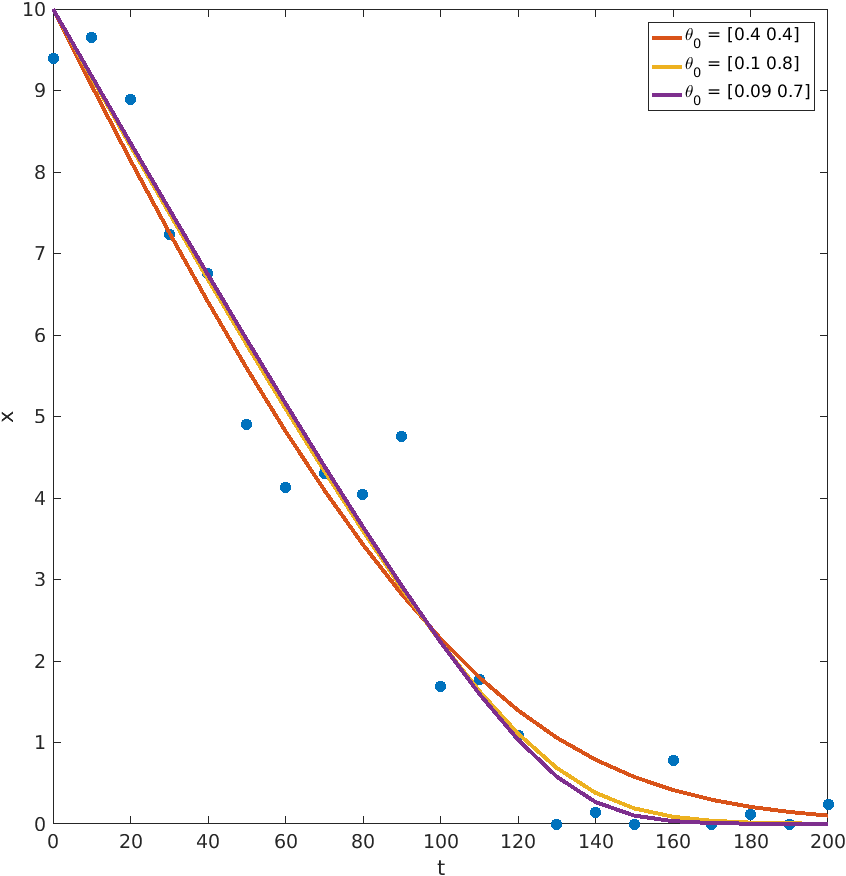
\includegraphics[width=0.55\textwidth]{../img/2-3}
\caption{Solutions for Trust Region Reflective algorithm using Jacobian, with default parameters}
\label{fig:2-3}
\end{figure}

In a nutshell, both TRR and LM converged to almost identical parameter estimates when the starting point was near the optimal solution. However, the LM algorithm failed to do so when started far away (see Table \ref{tab:2comparison}). Changing the step length and the stopping criteria did not make a difference in either algorithm. Our results indicate that the TRR algorithm performs better than the LM for this problem presumably because it is not underdetermined and its solution is bounded. As a result, we will focus on \texttt{lsqnonlin} set with TRR hereafter. 


In terms of the big picture, a lot of stable points (i.e. solutions) can be found for this system, which are represented by the yellow line. The starting guess "rolls down" straight onto the yellow line when finding an optimal solution. Therefore, this tells us that the value of $\theta^*$ depends largely on the initial starting guess. 

Figure \ref{fig:2-3} shows the resulting model for each of the starting guesses (set with TRR) along with their predictions and the observational data. It is evident that despite different starting guesses, the estimated $\theta_1$ values are very similar. On the other hand, the $\theta_2$ estimates varied more. The effect of the latter can be seen for high values of $t$ ($t\in 120-200$) where the model predictions become more convex (towards the data point cluster) for initial guesses that started closer to the optimal solution. 

Table \ref{tab:2-3stats} lists the $95\%$ confidence intervals of the parameter estimates. Notice that the confidence bounds are much narrower for the models with starting guesses closer to the optimal solution. 

In conclusion, our results indicate that TRR performs better than LM for this nonlinear least squares problem. Further, we learned that the starting initial guess has an influence on the resulting parameter estimate and their uncertainty. Optimization tasks with objective functions similar to the problem analyzed in this report should therefore pay importance to the choice of numerical algorithm and starting initial guess to obtain better results.  

\vspace*{\fill} 
\begin{table}[htbp]
\centering
\footnotesize
\begin{tabular}{l|ccc|cc} \hline \hline 
\multicolumn{6}{c}{$\theta_0 = [0.4\ 0.4]$} \\ \hline \hline
Parameter & Estimate & Lower bound & Upper bound & \multicolumn{2}{c}{Covariance}  \\& & & & $\theta_1$ & $\theta_2$ \\ \hline 
$\theta_1$ & 0.13 & 0.07 & 0.18 & 0.00 & \\ 
$\theta_2$ & 3.43 & -0.15 & 7.02 & -0.04 & 2.93 \\ 
\hline \hline 
\multicolumn{6}{c}{$\theta_0 = [0.1\ 0.8]$} \\ \hline \hline
Parameter & Estimate & Lower bound & Upper bound & \multicolumn{2}{c}{Covariance}  \\& & & & $\theta_1$ & $\theta_2$ \\ \hline 
$\theta_1$ & 0.09 & 0.07 & 0.12 & 0.00 & \\ 
$\theta_2$ & 1.08 & -0.13 & 2.28 & -0.01 & 0.33 \\ 
\hline \hline 
\multicolumn{6}{c}{$\theta_0 = [0.09\ 0.7]$} \\ \hline \hline
Parameter & Estimate & Lower bound & Upper bound & \multicolumn{2}{c}{Covariance}  \\& & & & $\theta_1$ & $\theta_2$ \\ \hline 
$\theta_1$ & 0.09 & 0.07 & 0.11 & 0.00 & \\ 
$\theta_2$ & 0.75 & -0.19 & 1.69 & -0.00 & 0.20 \\ 
\hline \hline 
\end{tabular} 

\caption{Parameter estimates, their covariance matrix, along with their $95\%$ confidence intervals are listed above for three different starting guesses. The parameters are estimated using \texttt{lsqnonlin} set with the Trust Region Reflective numerical algorithm.}
\label{tab:2-3stats}
\end{table}
\vspace*{\fill} 
